%! TeX program = lualatex
\documentclass[12pt]{article}

\usepackage{cmap}
\usepackage{minted}
\usepackage{caption}

\setminted{
    linenos,                % показывать номера строк
    breaklines,             % переносить длинные строки
    breakanywhere=true,     % переносить в любом месте
    tabsize=2,              % размер табуляции
    fontsize=\scriptsize,        % размер шрифта
    frame=lines,            % рамка сверху и снизу
    framesep=2mm,           % расстояние текста от рамки
    baselinestretch=1.1,    % межстрочный интервал
    autogobble=true,        % автоудаление общего отступа
    % xleftmargin=10pt,       % отступ слева
    % numbersep=5pt,          % расстояние между номерами и кодом
}

\usepackage[english, russian]{babel}

\usepackage[nopatch=footnote]{microtype}

\usepackage{float}
\usepackage{fontspec}
\usepackage[pdfborder={0 0 0}]{hyperref}

\usepackage{enumitem}

\setmainfont{TimesNewerRoman}[
  Extension = .otf,
  Path = /nix/store/ihdqrn4p54awd89vrday9k53s8i47bbv-times-newer-roman-unstable-2018-09-11/share/fonts/opentype/,
  UprightFont = *-Regular,
  BoldFont = *-Bold
]
\setmonofont{Ubuntu Mono}

\newcommand{\icon}[1]{\fontspec{UbuntuNerdFont}[Extension = .ttf,
  Path = /nix/store/h721jafy2n74x4k5p0hxbz722h0rncmx-nerd-fonts-ubuntu-3.3.0+0.83/share/fonts/truetype/NerdFonts/Ubuntu/,
  UprightFont = *-Regular,
BoldFont = *-Bold] #1}

\newcommand{\iicon}[1]{{\icon{#1}}}

\usepackage{graphicx}
\usepackage{fontawesome5} % Для иконок

\usepackage[left=2.0cm, right=2.0cm, top=1.0cm, bottom=1.0cm, includeheadfoot]{geometry}

% \usepackage[mocha, textcolor=true, pagecolor=true]{catppuccinpalette} \usemintedstyle{catppuccin-mocha}
\usepackage[latte, textcolor=true, pagecolor=true]{catppuccinpalette} \usemintedstyle{catppuccin-latte}

\usepackage{setspace}
\onehalfspacing

\usepackage{fancyhdr}
\fancyhf{}

\renewcommand{\sectionmark}[1]{\markboth{#1}{}}
\renewcommand{\subsectionmark}[1]{\markright{#1}}

% Настройка колонтитулов
\fancyhead[RO]{\rightmark}
\fancyhead[LO]{\leftmark}

\fancyfoot[L]{\hspace{8pt} \rule{\textwidth}{0.4pt}}
\fancyfoot[R]{\LARGE{\thepage}}
\fancyfoot[C]{}

\newcommand{\lablogo}
{
\begin{center}
    \huge{\textbf{Лабораторная работа №3}} \\
\end{center}
}

\newcommand{\colorURL}[1]{\textcolor{CtpBlue}{#1}}
\newcommand{\colorGIT}[1]{\textcolor{CtpLavender}{#1}}
\renewcommand{\texttt}[1]{{\small\ttfamily #1}}

\setlength{\headheight}{15.2pt}

\DeclareCaptionLabelFormat{gostfigure}{Рисунок #2}
\captionsetup[figure]{labelformat=gostfigure, labelsep=endash}

\DeclareCaptionLabelFormat{gostlisting}{Листинг #2}
\captionsetup[listing]{labelformat=gostlisting, labelsep=endash}

\usepackage{amsmath}
\numberwithin{listing}{section}
\numberwithin{figure}{section}

\usepackage{tocloft}
\renewcommand{\cftsecleader}{\cftdotfill{\cftdotsep}}

\begin{document}
\pagestyle{empty}
\lablogo
\tableofcontents
\renewcommand\listoflistingscaption{Листинг}
\listoflistings

\newpage
\pagestyle{fancy}
\lablogo
\begin{center}
	\section
	 [Задание \ \texorpdfstring{\faScroll}{}]
	 {Задание \ \texorpdfstring{\faScroll}{}\protect\footnotemark}
\end{center}
\begin{enumerate}
	\item Реализовать оконное приложение (Windows Forms).
	\item Оконное приложение должно позволять создавать объекты, отображать список созданных объектов в табличной форме и выполнять поиск и удаление.
	\item Реализовать сериализацию и десериализацию классов в приложении.
	\item Сохранить наследование в классах (как в лабораторной работе №1)
	\item Сделать возможность добавления нового объекта для каждого класса
	\item Интерфейс приложения должен быть дополнен кнопками для сохранения и загрузки классов из XML файлов.
	\item Операции сохранения и загрузки XML файлов должны быть выполнены с использованием методов async и await.
	\item Поиск данных должен выполняться для каждого класса отдельно
	\item Реализовать удаление данных (сохраняя верный порядок строк)
\end{enumerate}

\footnotetext{Варианты заданий в соответствии с вариантом лабораторной работы № 1}

\newpage
\begin{center}
	\subsection
	[Дополнительные задания~\texorpdfstring{\faLightbulb}{}]
	{Дополнительные задания~\texorpdfstring{\faLightbulb}{}\protect\footnotemark}
	\begin{minipage}{0.8\linewidth}
		\begin{enumerate}[noitemsep,topsep=0pt, left=0pt]
			\item[\faStar] Возможность изменения темы интерфейса
			      \begin{itemize}
				      \item Добавить выбор цветовой схемы (светлая или тёмная тема).
				      \item Использовать Flat стиль кнопок для современного вида.
			      \end{itemize}
			\item[\faSearch] Улучшенный поиск
			      \begin{itemize}
				      \item Реализовать фильтрацию данных в DataGridView в реальном времени (например, при вводе текста в TextBox).
				      \item Поиск с подсветкой найденных результатов.
			      \end{itemize}
			\item[\iicon{}] Контекстное меню
			      \begin{itemize}
				      \item Добавить правый клик на строку в \texttt{DataGridView}, чтобы появлялось меню с опциями (Редактировать или Удалить).
			      \end{itemize}
			\item[\iicon{}] Автосохранение
			      \begin{itemize}
				      \item Автоматически сохранять данные в XML при закрытии программы.
				      \item Загружать последние данные при запуске.
			      \end{itemize}
			\item[\iicon{}] Drag \& Drop
			      \begin{itemize}
				      \item Сделать так, чтобы XML-файлы можно было просто перетаскивать в окно приложения для загрузки.
			      \end{itemize}
			\item[\iicon{}] Экспорт в другие форматы
			      \begin{itemize}
				      \item Позволить сохранять данные не только в XML, но и в JSON.
			      \end{itemize}
			\item[\iicon{}] Статистика
			      \begin{itemize}
				      \item Добавить внизу статус-бар с инфо: "Объектов в базе: X".
			      \end{itemize}
			\item[\iicon{}] Логирование ошибок
			      \begin{itemize}
				      \item Если что-то пошло не так (ошибки при загрузке XML), выводить понятное сообщение пользователю.
			      \end{itemize}
			\item[\iicon{󰙨}] Генерация тестовых данных
			      \begin{itemize}
				      \item Добавить кнопку ''Сгенерировать тестовые данные'' для удобства тестирования.
			      \end{itemize}
			\item[\iicon{}] Горячие клавиши
			      \begin{itemize}
				      \item Например, Ctrl + S для сохранения, Ctrl + O для загрузки, Esc для очистки формы.
			      \end{itemize}
		\end{enumerate}
	\end{minipage}
\end{center}
\footnotetext{Дополнительные задания выполняются по желанию и не подлежат проверке на зачёте.}

\newpage

\section{Шаг 1. Создание проекта \ \texorpdfstring{{\small{\iicon{󰙴}}}}{}}
\begin{itemize}
	\item "Создать проект"
	\item "Windows forms(Майкрософт)" (Рисунок~\ref{fig:Обозначения разделов})
\end{itemize}

\begin{figure}[H]
	\centering
	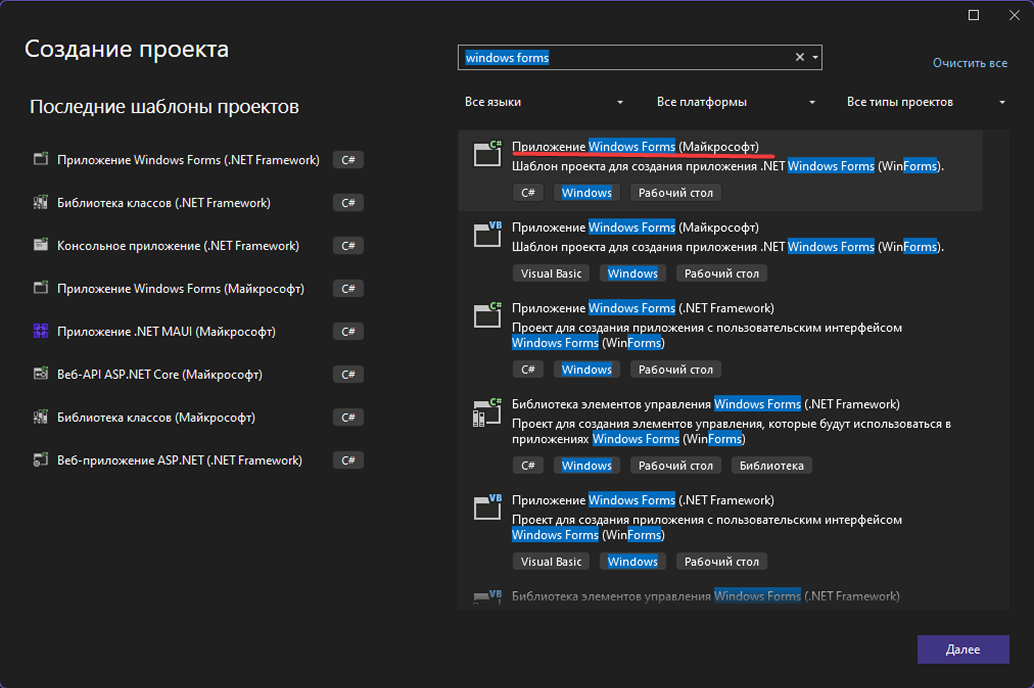
\includegraphics[width=0.6\textwidth]{fig/image-3.jpg}
	\caption{Обозначения разделов}
	\label{fig:Обозначения разделов}
\end{figure}

\begin{itemize}
	\item Указываете название формы (содержащее номер лабораторной работы)
	\item Выбираете последнюю версию платформы из доступных (в примере .NET 8.0) (Рисунок~\ref{fig:Настройки проекта})
\end{itemize}

\begin{figure}[H]
	\centering
	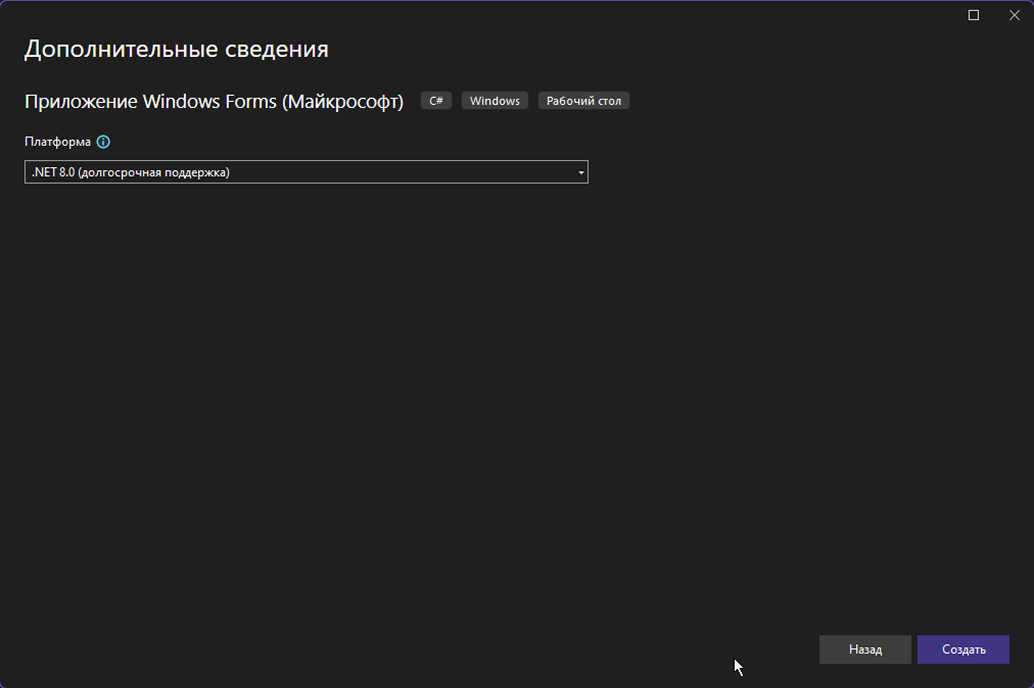
\includegraphics[width=0.6\textwidth]{fig/image-2.jpg}
	\caption{Обозначения разделов}
	\label{fig:Настройки проекта}
\end{figure}

Перед вами откроется проект с формой по умолчанию
Слева будет “Панель элементов” (если ее нет перейти в “Вид” \iicon{} “Панель элементов” / \texttt{Ctrl + Alt + X}) (Рисунок~\ref{fig:Окно проекта})

\begin{figure}[H]
	\centering
	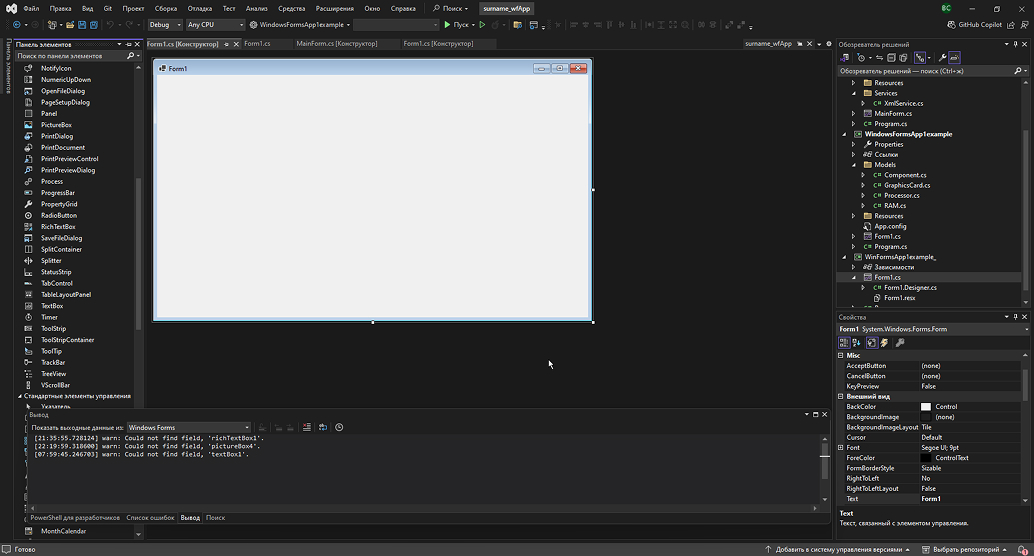
\includegraphics[width=0.8\textwidth]{fig/image-1.jpg}
	\caption{Окно проекта}
	\label{fig:Окно проекта}
\end{figure}

\newpage

\section{Основные элементы Windows Forms}
Панель элементов содержит множество элементов для работы с формами.
Можно выделить наиболее часто используемые:
\begin{itemize}
	\item \textbf{\texttt{Form:}}
	      Основное окно приложения. Служит контейнером для других элементов управления, предоставляет базовую функциональность для создания пользовательского интерфейса (размещение, масштабирование, обработка событий формы).
	\item \textbf{\texttt{Button:}}
	      Кнопка, по нажатию на которую происходит выполнение заданного кода. Используется для инициирования действий (например, отправка данных, переход на другую форму).
	\item \textbf{\texttt{Label:}}
	      Элемент для отображения текста. Предназначен для вывода информационных сообщений, описания других элементов и инструкций. Не поддерживает ввод данных.
	\item \textbf{\texttt{TextBox:}}
	      Поле для ввода и отображения однострочного текста. Используется для сбора пользовательского ввода, поиска, ввода паролей (с установкой \texttt{PasswordChar}) и т.д.
	\item \textbf{\texttt{RichTextBox:}}
	      Расширенная версия TextBox, позволяющая форматировать текст (изменять шрифты, цвета, стили). Полезна для редактирования многострочного форматированного текста.
	\item \textbf{\texttt{CheckBox:}}
	      Флажок, позволяющий выбирать или снимать выбор (логическое значение \texttt{true} или \texttt{false}). Применяется в формах для подтверждения, включения настроек и т.п.
	\item \textbf{\texttt{ListBox:}}
	      Список, позволяющий отображать набор элементов, из которых пользователь может выбрать один или несколько. Простой способ представления данных в виде списка.
	\item \textbf{\texttt{ComboBox:}}
	      Комбинированный элемент, который сочетает в себе поле для ввода и выпадающий список. Удобен для выбора одного значения из набора, позволяя пользователю как выбрать из списка, так и ввести значение вручную.
	\item \textbf{\texttt{ListView:}}
	      Многофункциональный список с поддержкой различных видов отображения (иконки, подробности, плитка). Позволяет отображать элементы с подэлементами, а также использовать возможности сортировки и фильтрации (но редактирование ограничено).
	\item \textbf{\texttt{DataGridView:}}
	      Табличное представление данных с поддержкой привязки данных, сортировки, фильтрации и встроенного редактирования ячеек.
	\item \textbf{\texttt{PictureBox:}}
	      Элемент для отображения изображений. Поддерживает различные форматы, позволяет масштабировать или изменять размер изображения в соответствии с настройками.
	\item \textbf{\texttt{Panel:}}
	      Контейнер для других элементов управления, позволяющий группировать связанные элементы и управлять их компоновкой. Может использоваться для создания сложных макетов или динамического отображения или скрытия групп элементов.
	\item \textbf{\texttt{GroupBox:}}
	      Контейнер с рамкой и заголовком, предназначенный для группировки элементов управления, которые логически связаны между собой. Улучшает визуальную организацию интерфейса.
	\item \textbf{\texttt{MenuStrip:}}
	      Панель меню, располагаемая обычно в верхней части формы. Позволяет создавать выпадающие меню (например, Файл, Правка, Вид и т.д.) для доступа к командам приложения.
	\item \textbf{\texttt{ToolStrip:}}
	      Панель инструментов, содержащая кнопки, текстовые поля, комбобоксы и другие элементы, предназначенные для быстрого доступа к функциям приложения.
	\item \textbf{\texttt{StatusStrip:}}
	      Элемент, располагаемый в нижней части формы, для отображения статусной информации (например, индикаторы, сообщения, время работы).
	\item \textbf{\texttt{TabControl:}}
	      Элемент, позволяющий создавать вкладки для организации контента в пределах одного окна. Удобен для разделения функциональности на логически связанные секции.
\end{itemize}

\newpage

\section{Шаг 2. Создание формы \ \texorpdfstring{{\small{\iicon{}}}}{}}
Для примера будет разработана форма содержащая следующие элементы:
\begin{enumerate}
	\item DatagridView - для добавления элементов и отображения их в табличном виде
	\item Button - для добавления элементов, удаления, и поиска
	\item TextBox - для ввода необходимых данных при добавлении элемента или поиска
	\item PictureBox - для добавления изображения
	\item Panel - для группировки элементов, создания “вкладок”
	\item Label - для подписи элементов
\end{enumerate}

Необходимо разместить соответствующие элементы на форме (пока что схематично). Пример формы изображен на рисунке~\ref{fig:Пример оформления формы}.

\begin{figure}[H]
	\centering
	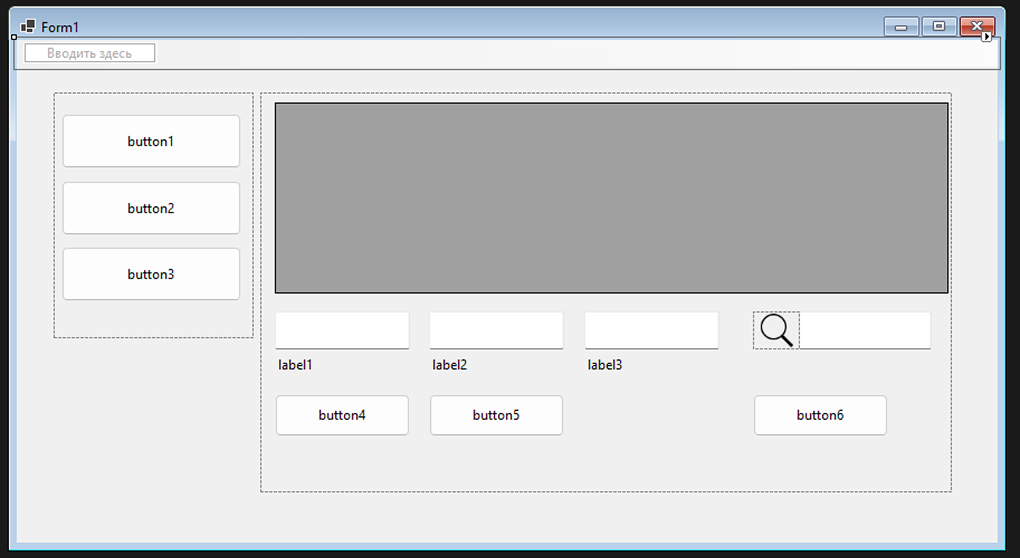
\includegraphics[width=0.8\textwidth]{fig/image.jpg}
	\caption{Пример оформления формы}
	\label{fig:Пример оформления формы}
\end{figure}

Возращаясь к настройке внешнего вида формы необходимо рассмотреть свойства элементов формы. В правом нижнем углу в проекте можно увидеть окно свойств элемента. Рассмотрим основные свойства, настройка которых потребуется для создания интуитивного и понятного интерфейса, а также изменения внешнего вида элементов.
В верхней части панели есть кнопки для сортировки и перехода по разделам (свойства, эффекты). Для того, чтобы быстрее найти нужное свойство можно выбрать сортировку “по категориям”.
Для того, чтобы изменить название элемента в коде (при обращении к нему, вызове метода) используется свойство (\texttt{Name}). Его можно найти в разделе “Design” (“Разработка”) (Рисунок~\ref{fig:Свойство Name}).

\begin{figure}[H]
	\centering
	
\includegraphics[width=0.8\textwidth]{fig/none.png}
	\caption{Свойство \texttt{Name}\protect\footnotemark}
	\label{fig:Свойство Name}
\end{figure}
\footnotetext{Подробно про свойства можно почитать по ссылке: \url{https://metanit.com/sharp/windowsforms/2.2.php}}

Для того, чтобы изменить текст, отображаемый на элементе, необходимо указать новое название в свойстве “\texttt{Text}” в разделе “Внешний вид” (Рисунок~\ref{fig:Свойство text})

\begin{figure}[H]
	\centering
	
\includegraphics[width=0.8\textwidth]{fig/none.png}
	\caption{Свойство Text}
	\label{fig:Свойство text}
\end{figure}

Также можно использовать своство \texttt{PlaceholderText}, чтобы изменить текст, отображаемый на элементе. Свойство находится в разделе “Misc” (Рисунок~\ref{fig:Свойство Placeholder}). Данное свойство доступно при создании проекта Майкрософт

\begin{figure}[H]
	\centering
	
\includegraphics[width=0.8\textwidth]{fig/none.png}
	\caption{Свойство \texttt{Placeholder}}
	\label{fig:Свойство Placeholder}
\end{figure}

Также необходимо настроить внещний вид элемента TextBox. Для того, чтобы изменить высоту TextBox, необходимо изменить значение праметра \texttt{Multiline} на True (Рисунок~\ref{fig:Свойство Multiline})


\begin{figure}[H]
	\centering
	
\includegraphics[width=0.8\textwidth]{fig/none.png}
	\caption{Свойство \texttt{Multiline}}
	\label{fig:Свойство Multiline}
\end{figure}

Для изменения фонового цвета используется свойство \texttt{BackColor}, а для изменения цвета текста - \texttt{ForeColor} (Рисунок~\ref{fig:Свойства для изменения цвета})


\begin{figure}[H]
	\centering
	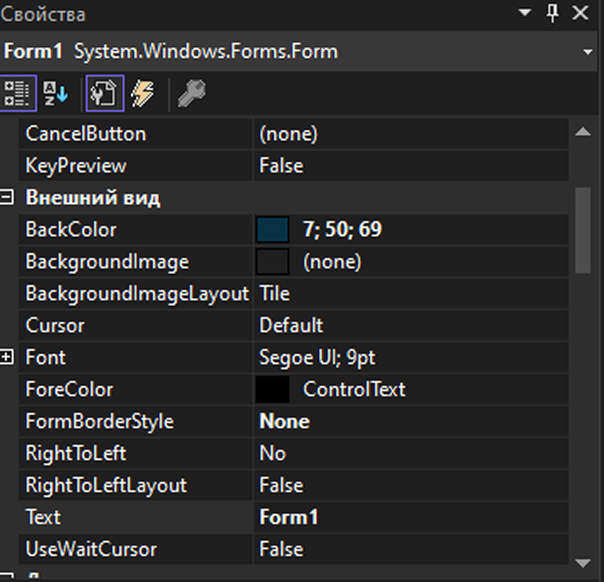
\includegraphics[width=0.6\textwidth]{fig/image 58.jpg}
	\caption{Свойства для изменения цвета}
	\label{fig:Свойства для изменения цвета}
\end{figure}

Применив необходимые изменения, получим форму, изображенную на рисунке~\ref{fig:Стилизация интерфейса на ваше умотрение smileface}

\begin{figure}[H]
	\centering
	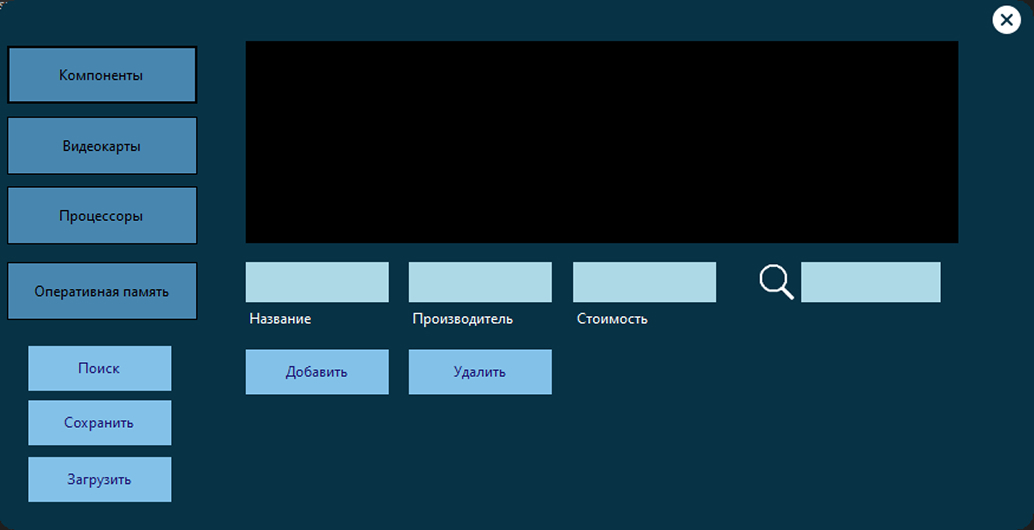
\includegraphics[width=0.8\textwidth]{fig/image 37.jpg}
	\caption{Пример стилизованной формы\protect\footnotemark}
	\label{fig:Стилизация интерфейса на ваше умотрение smileface}
\end{figure}
\footnotetext{Стилизация интерфейса на ваше усмотрение {\scriptsize{\iicon{}}}}

Важно учесть расположение форм, которые в данном случае находятся друг над другом. Расположение панелей на форме указано на рисунке~\ref{fig:Структура формы}.

\begin{figure}[H]
	\centering
	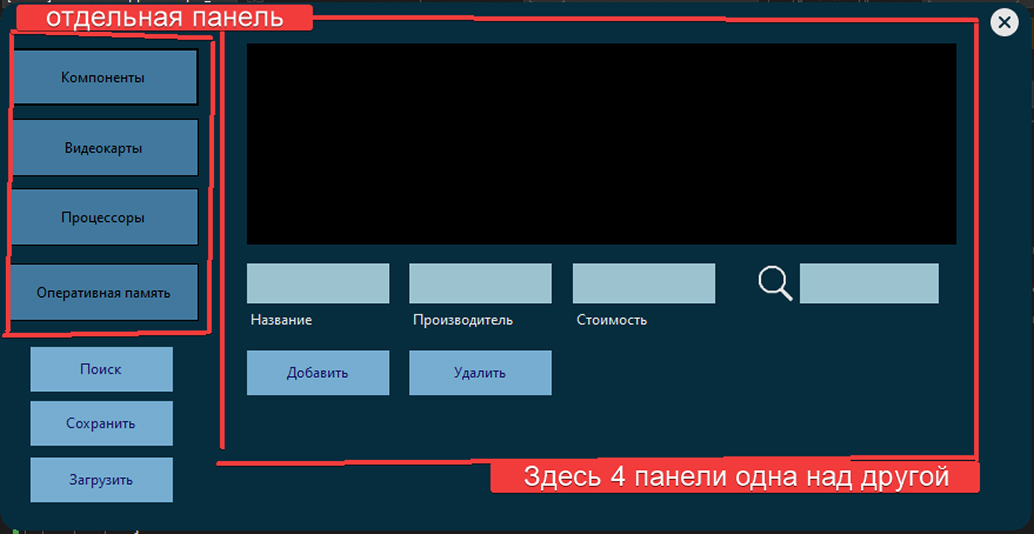
\includegraphics[width=0.8\textwidth]{fig/image 38.jpg}
	\caption{Структура формы}
	\label{fig:Структура формы}
\end{figure}

Также для более детального рассмотрения и управления положением элементов на форме можно воспользоваться окном “Структура документа” (Вид \iicon{} Другие окна \iicon{} Структура документа ), для этого нужно открыть в файл с самой формой (\texttt{Form.cs}). Структура документа изображена на рисунке~\ref{fig:Структура формы2}

\begin{figure}[H]
	\centering
	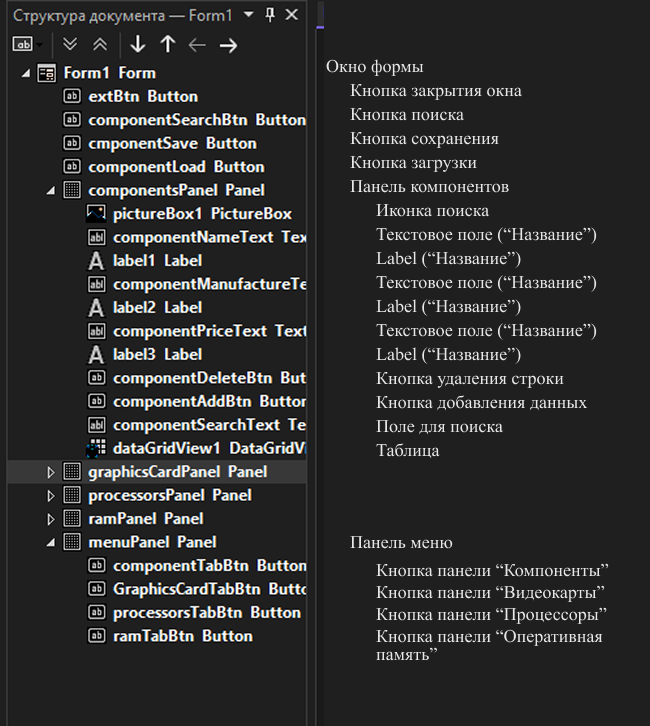
\includegraphics[width=0.6\textwidth]{fig/Group 98.jpg}
	\caption{Структура формы}
	\label{fig:Структура формы2}
\end{figure}

\newpage

\section{Шаг 3. Добавление классов \ \texorpdfstring{{\small{\iicon{}}}}{}}

Далее необходимо в Решении создать папку и добавить туда классы из лабораторной 1 (Рисунок~\ref{fig:Создание классов для работы с данными в форме})

\begin{figure}[H]
	\centering
	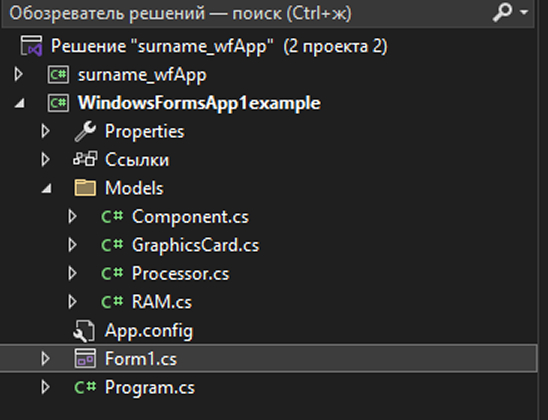
\includegraphics[width=0.6\textwidth]{fig/image 5.jpg}
	\caption{Создание классов для работы с данными в форме}
	\label{fig:Создание классов для работы с данными в форме}
\end{figure}

В каждом классе необходимо наличие 3 свойств, конструктора без параметров (нужен для сериализации) и конструктора с параметрами (Рисунок~\ref{lst:OrderCs}).

\begin{listing}[H]
	\inputminted[firstline = 9]{csharp}{../../2lab/surname_wfApp/Models/Component.cs}
	\caption{Пример структуры класса}
	\label{lst:OrderCs}
\end{listing}

\newpage

\section{Шаг 4. Реализация добавления данных в таблицу \ \texorpdfstring{{\small{\iicon{}}}}{}}

После добавления классов необходимо настроить обработчики событий.
В \texttt{WinForms} у элементов управления (кнопок, чекбоксов, текстовых полей и т. д.) есть события (\texttt{events}), которые вызываются при определенных действиях пользователя.
Например, клик по кнопке является одним из событий и при настройке появляется в окне свойств (Рисунок~\ref{fig:Добавление событий})

\begin{figure}[H]
	\centering
	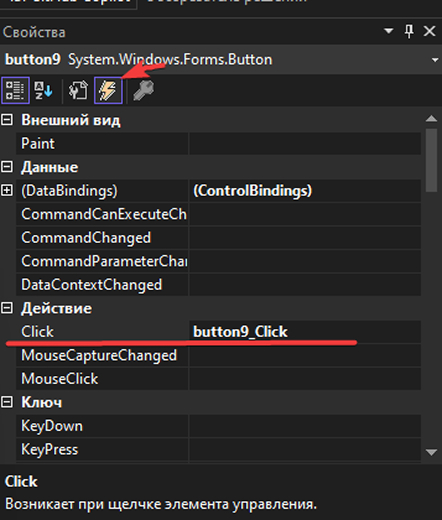
\includegraphics[width=0.6\textwidth]{fig/image 31.jpg}
	\caption{Добавление событий}
	\label{fig:Добавление событий}
\end{figure}

Если настраиваемое событие не отрабатывает, необходимо проверить панель свойств на наличие события в данном разделе.

Далее необходимо добавить событие нажатия на кнопку добавления данных в таблицу. Пример метода для добавления данных в форму представлен на рисунке~\ref{lst: Методы добавления данных в форму}

\begin{listing}[H]
	\inputminted[firstline = 162, lastline=196]{csharp}{../../2lab/WinFormsApp1example_/Form1.cs}
	\caption{Метод добавления данных в форму}
	\label{lst: Методы добавления данных в форму}
\end{listing}

Также необходимо после добавления данных обновить данные в таблице (\texttt{DataGridView}) (Рисунок~\ref{lst:Метод обновления Datagridview})

\begin{listing}[H]
	\inputminted[firstline = 230, lastline=273]{csharp}{../../2lab/WinFormsApp1example_/Form1.cs}
	\caption{Метод обновления \texttt{Datagridview}}
	\label{lst:Метод обновления Datagridview}
\end{listing}


Можно также добавить событие удаления элемента (строки) из таблицы (Рисунок~\ref{lst:Метод удаления строки из Datagridview} )

\begin{listing}[H]
	\inputminted[firstline = 342, lastline=359]{csharp}{../../2lab/WinFormsApp1example_/Form1.cs}
	\caption{Метод удаления строки из \texttt{Datagridview}}
	\label{lst:Метод удаления строки из Datagridview}
\end{listing}

Для добавления данных в заранее созданные поля, необходимо связать название поля с свойствами создаваемого объекта (Рисунок~\ref{lst:Добавления данных в столбцы DataGridView без автогенерации})

\begin{listing}[H]
	\inputminted[firstline=138, lastline=155]{csharp}{../../2lab/WinFormsApp1example_/Form1.cs}
	\caption{Добавления данных в столбцы \texttt{DataGridView} без автогенерации}
	\label{lst:Добавления данных в столбцы DataGridView без автогенерации}
\end{listing}

Важно при работе с панелями динамически скрывать и делать их видимыми при выборе соответствующей вкладки. Для этого необходимо создать метод, который будет менять свойство \texttt{Visible} у соответсвущей панели при нажатии на кнопку (Рисунок~\ref{lst:Метод скрытия панелей})

\begin{listing}[H]
	\inputminted[firstline = 100, lastline=131]{csharp}{../../2lab/WinFormsApp1example_/Form1.cs}
	\caption{Метод скрытия панелей}
	\label{lst:Метод скрытия панелей}
\end{listing}

\newpage

\section{Шаг 5. Реализация фильтрации (поиска) данных \ \texorpdfstring{{\small{\iicon{}}}}{}}
Для поиска нужных данных в таблице использует поиск по подстроке в каждом столбце (листинг~\ref{lst:Метод фильтрации (поиска) данных в таблице}).

\begin{listing}[H]
	\inputminted[firstline = 280, lastline=341, fontsize={\fontsize{8}{8}}]{csharp}{../../2lab/WinFormsApp1example_/Form1.cs}
	\caption{Метод фильтрации (поиска) данных в таблице}
	\label{lst:Метод фильтрации (поиска) данных в таблице}
\end{listing}

\newpage

\section{Шаг 6. Сериализация, десериализация классов. Сохранение в XML \ \texorpdfstring{{\small{\iicon{}}}}{}}

\textbf{Сериализация} -- это процесс преобразования объекта в поток байтов для его сохранения в файле, передаче по сети или хранении в базе данных. Впоследствии этот объект можно восстановить (десериализовать).

Типы сериализации в C\#

В C\# есть несколько типов сериализации
\begin{itemize}
	\item \textbf{Binary} (Бинарная) — сериализация в двоичный формат (быстро, но неудобно для чтения)
	\item \textbf{XML} (Текстовая) — сохраняет объект в формате XML (читаемый формат, но объемный)
	\item \textbf{JSON} (Современный стандарт) — сериализация в JSON (удобно для веба, поддерживается большинством языков)
	\item \textbf{Custom} (Кастомная) — своя реализация, например, в CSV\footnote{Это простой текстовый формат для хранения табличных данных, где каждая строка файла представляет одну строку таблицы. Значения в каждой строке разделяются определенным символом, чаще всего запятой.}.
\end{itemize}

В данном случае будет рассмотрена XML-сериализация. В C\# для работы с XML используется класс \texttt{XmlSerializer} из пространства имен \texttt{System.\-Xml.\-Serialization}.

% NOTE delete?
% \textbf{XML} (Extensible Markup Language) — это читаемый человеком формат, используемый для хранения структурированных данных.

Пример метода сериализации с использованием \texttt{List} приведен на рисунке~\ref{lst:Пример метода сериализации классов}

% \begin{listing}[H]
\inputminted[firstline = 531, lastline=598]{csharp}{../../2lab/WinFormsApp1example_/Form1.cs}
% \captionof{listing}{Пример сериализации данных с помощью \texttt{DataTable}}
\label{lst:Пример метода сериализации классов}
% \end{listing}


Объяснение ключевых моменто
\begin{itemize}
	\item \textbf{\texttt{SaveFileDialog:}}
	      Используется для взаимодействия с пользователем, чтобы выбрать место и имя файла. Filter ограничивает выбор XML-файлами, но позволяет выбрать "все файлы" (\texttt{*.*:})
	\item \textbf{\texttt{XmlSerializer:}}
	      Инструмент для преобразования объектов C\# (в данном случае списков \texttt{List<T>}) в XML-формат и обратно. Он требует, чтобы классы (\texttt{Component, GraphicsCard, Processor}) имели публичные свойства и пустой конструктор
	\item \textbf{\texttt{using (TextWriter ...):}}
	      Обеспечивает корректное закрытие файла после записи, даже если произойдёт ошибка
	\item \textbf{\texttt{Проверка на пустой список:}}
	      Перед сериализацией проверяется \texttt{Count}, чтобы не создавать пустой XML-файл
	\item \textbf{\texttt{Условные ветви (if-else):}}
	      Код определяет, какой список сериализовать, основываясь на активном \texttt{DataGridView}. Это позволяет сохранять данные только для текущей вкладки.
\end{itemize}

Также можно использовать сериализацию данных с помощью \texttt{DataTable}, не используя списки \texttt{List} (Рисунок~\ref{fig:Серилилация данных через DataTable})

% NOTE такого кода нету 
\begin{listing}[H]
	\inputminted[firstline = 531, lastline=550]{csharp}{../../2lab/WinFormsApp1example_/Form1.cs}
	\captionof{listing}{Пример сериалазации данных с помощью \texttt{DataTable}}
	\label{fig:Серилилация данных через DataTable}
\end{listing}

\begin{listing}[H]
	\inputminted[firstline = 467, lastline=521, fontsize={\fontsize{8}{8.5}}]{csharp}{../../2lab/WinFormsApp1example_/Form1.cs}
	% TODO: убрать footnote из listinglist
	\captionof{listing}{Пример метода десериализации\protect\footnotemark}
\end{listing}

\footnotetext{Десериализация — это процесс обратного преобразования, то есть восстановления объекта из сохраненного состояния}

\noindent Разбор метода десериализации


\begin{listing}[H]
	\inputminted[firstline = 467, lastline=468]{csharp}{../../2lab/WinFormsApp1example_/Form1.cs}
	\captionof{listing}{Метод десериализации с параметром}
	\label{lst:method dis}
\end{listing}

Метод принимает параметр \texttt{dgv} типа \texttt{DataGridView}, чтобы знать, в какой \texttt{DataGridView} нужно загрузить данные (например, \texttt{dataGridView4} для процессоров, \texttt{dataGridView1} для компонентов или \texttt{dataGridView2} для видеокарт). Такой подход делает метод универсальным — он может работать с любым DataGridView, а не с конкретным. Это удобно, если у вас несколько таблиц (\texttt{dataGridView1}, \texttt{dataGridView2}, \texttt{dataGrid\-View4}), и вы хотите переиспользовать код. (Рисунок~\ref{lst:method dis})

\begin{listing}[H]
	\inputminted[firstline = 470, lastline=472]{csharp}{../../2lab/WinFormsApp1example_/Form1.cs}
	\captionof{listing}{Объект \texttt{OpenFileDialog}}
	\label{lst:OpenFileDialog}
\end{listing}

Создаётся объект \texttt{OpenFileDialog} для выбора файла пользователем. Свойство \texttt{Filter} задаёт фильтр файлов, чтобы в диалоге отображались только XML-файлы по умолчанию, но с возможностью выбрать "все файлы". Фильтр упрощает пользователю выбор нужного файла, показывая только файлы с расширением .xml.

Формат фильтра "XML Files (*.xml)|*.xml|All Files (*.*)|*.*" — это стандартный синтаксис для \texttt{OpenFileDialog}. Первая часть (XML Files (*.xml)) — это описание, вторая (*.xml) — маска файлов. Аналогично для "All Files". (Рисунок~\ref{lst:OpenFileDialog})

\begin{listing}[H]
	\inputminted[firstline = 474, lastline=482]{csharp}{../../2lab/WinFormsApp1example_/Form1.cs}
	\captionof{listing}{Выбор файла и проверка на корректную таблицу}
	\label{lst:table}
\end{listing}

Метод \texttt{ShowDialog()} (Рисунок~\ref{lst:table}) открывает диалоговое окно выбора файла. Если пользователь выбрал файл и нажал "Открыть", возвращается \texttt{DialogResult.OK}. Если пользователь нажал "Отмена", метод завершится, ничего не делая.

Свойство \texttt{FileName} возвращает полный путь к выбранному файлу (например, "\texttt{C:\textbackslash data.xml}"). Этот путь нужен для чтения данных из файла. Без пути не получится открыть файл для десериализации.

\begin{listing}
	\begin{minted}{csharp}
        if (dgv == null)
        {
            MessageBox.Show("Передан некорректный DataGridView для загрузки данных.");
            return;
        }
    \end{minted}
\end{listing}


Проверяется, что переданный \texttt{DataGridView} \texttt{(dgv)} не равен \texttt{null}. Если \texttt{dgv} равен \texttt{null}, дальнейшая работа с ним вызовет исключение \texttt{NullReferenceException}. Эта проверка защищает от таких ошибок.

\begin{listing}[H]
	\inputminted[firstline = 485, lastline=493]{csharp}{../../2lab/WinFormsApp1example_/Form1.cs}
	\captionof{listing}{Сериализация XML}
	\label{lst:ser XML}
\end{listing}

Далее рассмотрим объект \texttt{XMlSerializer}, позволяющий сохранять данные из таблицы в формате XML (Рисунок~\ref{lst:ser XML})

Если переданный \texttt{DataGridView} — это \texttt{dataGridView1} (для компонентов), данные загружаются в \texttt{componentList}

Создаётся объект \texttt{XmlSerializer} для типа \texttt{List<Component>}. \texttt{XmlSerializer} знает, как преобразовать XML в список объектов \texttt{Component}

указывает, что ожидается XML-файл, содержащий список объектов \texttt{Component}

\texttt{StreamReader} открывает файл по пути \texttt{filePath} для чтения текста
Конструкция \texttt{using} гарантирует, что поток (\texttt{StreamReader}) будет закрыт после использования, даже если произойдёт исключение

Метод \texttt{Deserialize} читает XML из потока и преобразует его в объект типа \texttt{List<Component>}
Приведение \texttt{(List<Component>)} необходимо, так как \texttt{Deserialize} возвращает объект типа \texttt{object}

Сбрасывается фильтр, чтобы после загрузки отображался полный список компонентов, а не отфильтрованный.

Этот блок загружает данные из XML-файла в список \texttt{componentList}, который привязан к \texttt{dataGr\-id\-View1}. Сброс фильтра (\texttt{filteredComponentList = null}) гарантирует, что пользователь увидит все загруженные данные.

Почему так: Использование \texttt{XmlSerializer} — это стандартный способ десериализации XML в .NET. Проверка \texttt{dgv == dataGridView1} позволяет методу работать с разными \texttt{DataGridView} и списками.
Также важно связать события кнопок сохранения и загрузки с соответствующими таблицами (Рисунок 6.8)

Рисунок 6.8 Связь событий и кнопок с помощью Tag

\newpage

\section{Дополнительная информация~\texorpdfstring{\iicon{}}{}}

\begin{enumerate}
	\item Обязательно ли указывать атрибут Serializable? \\
	      Нет, атрибут \texttt{[Serializable]} не нужен, если используется \texttt{DataSet} / \texttt{DataTable} + XML для сохранения данных.

	\item Почему Serializable не важен? \\
	      Атрибут \texttt{[Serializable]} требуется, если объекты сохраняются с помощью бинарной или JSON-сериализации (например, \texttt{BinaryFormatter} или \texttt{JsonSerializer}).

	      \textcolor{CtpRed}{НО} при использовании \texttt{DataSet.WriteXml(filePath)} не нужно указывать атрибут так как :
	      \begin{itemize}
		      \item \texttt{DataSet.WriteXml(filePath)} сохраняет данные в XML без необходимости сериализации класса.
		      \item Работает с таблицами (\texttt{DataTable}), а не с объектами конкретного \texttt{List}.
	      \end{itemize}

	      Когда \texttt{[Serializable]} был бы нужен
	      \begin{itemize}
		      \item Если объекты List сохраняются в файл (например, JSON, Binary, SOAP)
		      \item Если используется \texttt{BinaryFormatter} или \texttt{JsonConvert.\-Serialize\-Object(graphics\-Card\-List)}
	      \end{itemize}
\end{enumerate}

Если необходимо добавлять данные в уже созданные ячейки \texttt{DataGridView}, а не создавать новые строки, небходимо обновлять значения ячеек в существующих строках. Это можно сделать несколькими способами:

\begin{enumerate}
	\item Обращение к ячейкам по индексу строки и столбца

	      В случае, если в DataGridView уже присутствуют строки, можно обновлять данные так:

	      \begin{minted}{csharp}
                // Обновление данных в первой строке (индекс 0)
                dataGridView1.Rows[0].Cells[0].Value = "Новое значение";
                dataGridView1.Rows[0].Cells[1].Value = 123;
          \end{minted}

	\item Работа с \texttt{DataTable} (если \texttt{DataGridView} привязан к нему)

	      Если \texttt{DataGridView} использует \texttt{DataTable} как источник данных:

	      \begin{minted}{csharp}
                // Получаем доступ к DataTable
                DataTable dt = (DataTable)dataGridView1.DataSource; // Изменяем данные в нужной строке и столбце
                dt.Rows[0]["НазваниеСтолбца"] = "Новое значение";
          \end{minted}

	      После этого \texttt{DataGridView} обновится автоматически.

	\item Обновление данных через \texttt{BindingList<T>}

	      Если \texttt{DataGridView} привязан к \texttt{BindingList<T>}, можно менять объект в списке:

	      \begin{minted}{csharp}
                // Предположим, нас есть BindingList<MyObject> bindingList[0].SomeProperty =
                "Новое значение"; dataGridView1.Refresh();
                // Принудительно обновляем DataGridView
          \end{minted}
\end{enumerate}

\noindent \textcolor{CtpRed}{Важно:}
\begin{itemize}
	\item Убедись, что строки уже существуют перед обновлением (\texttt{dataGridView1.Rows.Count})
	\item Если \texttt{DataGridView} связан с \texttt{DataTable} или \texttt{BindingList<T>}, изменения надо делать в источнике данных.
\end{itemize}

\newpage

\section{Стилизация интерфейса~~\texorpdfstring{\iicon{}}{}}

Для того, чтобы убрать шапку формы используемую по умолчанию, необходимо установить значение \texttt{None} у свойства \texttt{FormBorderStyle} в разделе “Внешний вид” (Рисунок 6.9)

Рисунок 6.9 Свойство FormBorderStyle

После этого возможность перемещать форму с помощью мыши будет отключена. Чтобы вернуть возможность перемещения формы необходимо добавить флаги для реализации перемещения формы, функции для перемещения формы и обработчики событий нажатия мыши. Также можно стилизовать форму закруглив края с помощью функции \texttt{CreateRoundRectRgn}

Флаги для реализации перемещения формы и функции для перемещения формы, а также функции для скругления краев формы представлены на рисунке (Рисунок 6.10)

Рисунок 6.10 Функции реализации перемещения формы

Обработчики нажатия мыши приведены на рисунке 6.11

Рисунок 6.11 Обработчики движения мыши

Также в примере применяется изменение цвета элементов \texttt{label}, размещенных внутри \texttt{groupbox} Рисунок 6.12

Рисунок 6.12 Обработчики движения мыши

\newpage

\section{Форматирование данных~\texorpdfstring{\iicon{}}{}}
Для того, чтобы отформатировать данные в форме, например автоматически приводить стоимость к денежному формату (добавлять пробел, числа после запятой и знак валюты) необходимо добавить метод, который будет изменять содержимое соответствующего столбца (Рисунок 6.13, Рисунок 6.14)

Рисунок 6.13 Форматирование столбца \texttt{Price}

Рисунок 6.14 Метод форматирования строки с стоимостью
А затем вызывать этот метод у каждой таблицы (свойство \texttt{CellFormatting}) Рисунок 6.15

Рисунок 6.15 Вызов метода форматирования

\newpage
\section{Интерфейс приложения~~\texorpdfstring{\faGlasses}{}}

Далее представлены примеры интерфейса приложения.
Добавление данных в таблицу Components представлено на рисунке 6.16

Рисунок 6.16 Добавление данных в таблицу компонентов
Удаление осуществляется нажатием на соответствующую строку и затем нажатием кнопки “Удалить” (Рисунок 6.17)

Рисунок 6.17 Удаление данных из таблицы компонентов
Поиск осуществляется путем ввода данных в поле поиска и нажатием кнопки “Поиск”. Поля поиска в данном случае уникальные для каждой панели (класса), но кнопка поиска одна. (Рисунок 6.18)

Рисунок 6.18 Добавление данных в таблицу компонентов
Поиск осуществляется путем ввода данных в поле поиска и нажатием кнопки “Поиск”. Поля поиска в данном случае уникальные для каждой панели (класса), но кнопка поиска одна (Рисунок 6.19)

Рисунок 6.19 Добавление данных в таблицу компонентов
Также реализовано добавление данных в таблицы других классов (Рисунок 6.20)

Рисунок 6.20 Добавление данных в таблицу видеокарт

\newpage

\section{Вопросы для защиты~\texorpdfstring{\icon{}}{}}

\begin{enumerate}
	\item Вопрос
	\item Вопрос
	\item Вопрос
	\item Вопрос
	\item Вопрос
	\item Вопрос
	\item Вопрос
	\item Вопрос
	\item Вопрос
	\item Вопрос
\end{enumerate}

\end{document}
